\chapter{Evaluierung}
\label{chap:eval}
\todo[size=\small, color=blue!40, inline]{Kapitel: Evaluierung}%
\begin{itemize}
 \item wie skaliert das System / bringt es was?
 \item Cache löschen - neu laden -> Zeit messen
 \item Verschiedene Kamerapositionen:
 \begin{itemize}
  \item Turbine
  \item Cockpit
  \item Heck
  \item ``Businessclass''
  \item seitlich von Außen
 \end{itemize}
 \item Erklärung der Tests \& Diagramme
 \item Balancierung durch c-Collision Protokoll / die Varianz
\end{itemize}
\todo[size=\small, inline]{Grafiken mit echten Daten füllen!}%




%\begin{figure}
%\centering
%%%%%%%%%%%%%%%%%%%%%%%%%%%%%%%%%%%%%%%%%%%%%%%%%%%%%%%%%%
% Beispieldiagramm mit pgfplot und datenfile
%%%%%%%%%%%%%%%%%%%%%%%%%%%%%%%%%%%%%%%%%%%%%%%%%%%%%%%%%

\begin{tikzpicture}
  \begin{axis}[xlabel=Kameraposition, ylabel={Zeit (in Sekunden)}]
    \addplot table[col sep=comma,x index=0,y index=1,header=false] {data/ReloadTest_Redundance3_R2_D32.2010-1-25.log};
    %\addlegendentry{DataNode0}
    \addplot table[col sep=comma,x index=0,y index=2,header=false] {data/ReloadTest_Redundance3_R2_D32.2010-1-25.log};
    %\addlegendentry{DataNode1}
    \addplot table[col sep=comma,x index=0,y index=3,header=false] {data/ReloadTest_Redundance3_R2_D32.2010-1-25.log};
    %\addlegendentry{DataNode2}
    \addplot table[col sep=comma,x index=0,y index=4,header=false] {data/ReloadTest_Redundance3_R2_D32.2010-1-25.log};
    %\addlegendentry{DataNode3}
    \addplot table[col sep=comma,x index=0,y index=5,header=false] {data/ReloadTest_Redundance3_R2_D32.2010-1-25.log};
    %\addlegendentry{DataNode4}
    \addplot table[col sep=comma,x index=0,y index=6,header=false] {data/ReloadTest_Redundance3_R2_D32.2010-1-25.log};
    %\addlegendentry{DataNode5}
    \addplot table[col sep=comma,x index=0,y index=7,header=false] {data/ReloadTest_Redundance3_R2_D32.2010-1-25.log};
    %\addlegendentry{DataNode6}
    \addplot table[col sep=comma,x index=0,y index=8,header=false] {data/ReloadTest_Redundance3_R2_D32.2010-1-25.log};
    %\addlegendentry{DataNode7}
    \addplot table[col sep=comma,x index=0,y index=9,header=false] {data/ReloadTest_Redundance3_R2_D32.2010-1-25.log};
    %\addlegendentry{DataNode8}
    \addplot table[col sep=comma,x index=0,y index=10,header=false] {data/ReloadTest_Redundance3_R2_D32.2010-1-25.log};
    %\addlegendentry{DataNode9}
    \addplot table[col sep=comma,x index=0,y index=11,header=false] {data/ReloadTest_Redundance3_R2_D32.2010-1-25.log};
    %\addlegendentry{DataNode10}
    \addplot table[col sep=comma,x index=0,y index=12,header=false] {data/ReloadTest_Redundance3_R2_D32.2010-1-25.log};
    %\addlegendentry{DataNode11}
    \addplot table[col sep=comma,x index=0,y index=13,header=false] {data/ReloadTest_Redundance3_R2_D32.2010-1-25.log};
    %\addlegendentry{DataNode12}
    \addplot table[col sep=comma,x index=0,y index=14,header=false] {data/ReloadTest_Redundance3_R2_D32.2010-1-25.log};
    %\addlegendentry{DataNode13}
    \addplot table[col sep=comma,x index=0,y index=15,header=false] {data/ReloadTest_Redundance3_R2_D32.2010-1-25.log};
    %\addlegendentry{DataNode14}
    \addplot table[col sep=comma,x index=0,y index=16,header=false] {data/ReloadTest_Redundance3_R2_D32.2010-1-25.log};
    %\addlegendentry{DataNode15}
    \addplot table[col sep=comma,x index=0,y index=17,header=false] {data/ReloadTest_Redundance3_R2_D32.2010-1-25.log};
    %\addlegendentry{DataNode16}
    \addplot table[col sep=comma,x index=0,y index=18,header=false] {data/ReloadTest_Redundance3_R2_D32.2010-1-25.log};
    %\addlegendentry{DataNode17}
    \addplot table[col sep=comma,x index=0,y index=19,header=false] {data/ReloadTest_Redundance3_R2_D32.2010-1-25.log};
    %\addlegendentry{DataNode18}
    \addplot table[col sep=comma,x index=0,y index=20,header=false] {data/ReloadTest_Redundance3_R2_D32.2010-1-25.log};
    %\addlegendentry{DataNode19}
    \addplot table[col sep=comma,x index=0,y index=21,header=false] {data/ReloadTest_Redundance3_R2_D32.2010-1-25.log};
    %\addlegendentry{DataNode20}
    \addplot table[col sep=comma,x index=0,y index=22,header=false] {data/ReloadTest_Redundance3_R2_D32.2010-1-25.log};
    %\addlegendentry{DataNode21}
    \addplot table[col sep=comma,x index=0,y index=23,header=false] {data/ReloadTest_Redundance3_R2_D32.2010-1-25.log};
    %\addlegendentry{DataNode22}
    \addplot table[col sep=comma,x index=0,y index=24,header=false] {data/ReloadTest_Redundance3_R2_D32.2010-1-25.log};
    %\addlegendentry{DataNode23}
    \addplot table[col sep=comma,x index=0,y index=25,header=false] {data/ReloadTest_Redundance3_R2_D32.2010-1-25.log};
    %\addlegendentry{DataNode24}
    \addplot table[col sep=comma,x index=0,y index=26,header=false] {data/ReloadTest_Redundance3_R2_D32.2010-1-25.log};
    %\addlegendentry{DataNode25}
    \addplot table[col sep=comma,x index=0,y index=27,header=false] {data/ReloadTest_Redundance3_R2_D32.2010-1-25.log};
    %\addlegendentry{DataNode26}
    \addplot table[col sep=comma,x index=0,y index=28,header=false] {data/ReloadTest_Redundance3_R2_D32.2010-1-25.log};
    %\addlegendentry{DataNode27}
    \addplot table[col sep=comma,x index=0,y index=29,header=false] {data/ReloadTest_Redundance3_R2_D32.2010-1-25.log};
    %\addlegendentry{DataNode28}
    \addplot table[col sep=comma,x index=0,y index=30,header=false] {data/ReloadTest_Redundance3_R2_D32.2010-1-25.log};
    %\addlegendentry{DataNode29}
    \addplot table[col sep=comma,x index=0,y index=31,header=false] {data/ReloadTest_Redundance3_R2_D32.2010-1-25.log};
    %\addlegendentry{DataNode30}
    \addplot table[col sep=comma,x index=0,y index=32,header=false] {data/ReloadTest_Redundance3_R2_D32.2010-1-25.log};
    %\addlegendentry{DataNode31}
    \addplot table[col sep=comma,x index=0,y index=33,header=false] {data/ReloadTest_Redundance3_R2_D32.2010-1-25.log};
    %\addlegendentry{Average}
  \end{axis}
\end{tikzpicture}

%  \caption{Zeit zum Vollständigen Neuladen an einer Kameraposition. (Redundanz=3, 2 Renderer und 32 Datenknoten)}
%  \label{fig:eval:diag1}
%\end{figure}

%\begin{figure}
%\centering
%%%%%%%%%%%%%%%%%%%%%%%%%%%%%%%%%%%%%%%%%%%%%%%%%%%%%%%%%%
% Beispieldiagramm mit pgfplot und datenfile
%%%%%%%%%%%%%%%%%%%%%%%%%%%%%%%%%%%%%%%%%%%%%%%%%%%%%%%%%

\begin{tikzpicture}
  \begin{axis}[xlabel=Kameraposition, ylabel={Zeit (in Sekunden)}]
    \addplot+[only marks] table[col sep=comma,x index=0,y index=1,header=false] {data/ReloadTest_Redundance2_R2_D32.2010-1-26.log};
    %\addlegendentry{DataNode0}
    \addplot+[only marks] table[col sep=comma,x index=0,y index=2,header=false] {data/ReloadTest_Redundance2_R2_D32.2010-1-26.log};
    %\addlegendentry{DataNode1}
    \addplot+[only marks] table[col sep=comma,x index=0,y index=3,header=false] {data/ReloadTest_Redundance2_R2_D32.2010-1-26.log};
    %\addlegendentry{DataNode2}
    \addplot+[only marks] table[col sep=comma,x index=0,y index=4,header=false] {data/ReloadTest_Redundance2_R2_D32.2010-1-26.log};
    %\addlegendentry{DataNode3}
    \addplot+[only marks] table[col sep=comma,x index=0,y index=5,header=false] {data/ReloadTest_Redundance2_R2_D32.2010-1-26.log};
    %\addlegendentry{DataNode4}
    \addplot+[only marks] table[col sep=comma,x index=0,y index=6,header=false] {data/ReloadTest_Redundance2_R2_D32.2010-1-26.log};
    %\addlegendentry{DataNode5}
    \addplot+[only marks] table[col sep=comma,x index=0,y index=7,header=false] {data/ReloadTest_Redundance2_R2_D32.2010-1-26.log};
    %\addlegendentry{DataNode6}
    \addplot+[only marks] table[col sep=comma,x index=0,y index=8,header=false] {data/ReloadTest_Redundance2_R2_D32.2010-1-26.log};
    %\addlegendentry{DataNode7}
    \addplot+[only marks] table[col sep=comma,x index=0,y index=9,header=false] {data/ReloadTest_Redundance2_R2_D32.2010-1-26.log};
    %\addlegendentry{DataNode8}
    \addplot+[only marks] table[col sep=comma,x index=0,y index=10,header=false] {data/ReloadTest_Redundance2_R2_D32.2010-1-26.log};
    %\addlegendentry{DataNode9}
    \addplot+[only marks] table[col sep=comma,x index=0,y index=11,header=false] {data/ReloadTest_Redundance2_R2_D32.2010-1-26.log};
    %\addlegendentry{DataNode10}
    \addplot+[only marks] table[col sep=comma,x index=0,y index=12,header=false] {data/ReloadTest_Redundance2_R2_D32.2010-1-26.log};
    %\addlegendentry{DataNode11}
    \addplot+[only marks] table[col sep=comma,x index=0,y index=13,header=false] {data/ReloadTest_Redundance2_R2_D32.2010-1-26.log};
    %\addlegendentry{DataNode12}
    \addplot+[only marks] table[col sep=comma,x index=0,y index=14,header=false] {data/ReloadTest_Redundance2_R2_D32.2010-1-26.log};
    %\addlegendentry{DataNode13}
    \addplot+[only marks] table[col sep=comma,x index=0,y index=15,header=false] {data/ReloadTest_Redundance2_R2_D32.2010-1-26.log};
    %\addlegendentry{DataNode14}
    \addplot+[only marks] table[col sep=comma,x index=0,y index=16,header=false] {data/ReloadTest_Redundance2_R2_D32.2010-1-26.log};
    %\addlegendentry{DataNode15}
    \addplot+[only marks] table[col sep=comma,x index=0,y index=17,header=false] {data/ReloadTest_Redundance2_R2_D32.2010-1-26.log};
    %\addlegendentry{DataNode16}
    \addplot+[only marks] table[col sep=comma,x index=0,y index=18,header=false] {data/ReloadTest_Redundance2_R2_D32.2010-1-26.log};
    %\addlegendentry{DataNode17}
    \addplot+[only marks] table[col sep=comma,x index=0,y index=19,header=false] {data/ReloadTest_Redundance2_R2_D32.2010-1-26.log};
    %\addlegendentry{DataNode18}
    \addplot+[only marks] table[col sep=comma,x index=0,y index=20,header=false] {data/ReloadTest_Redundance2_R2_D32.2010-1-26.log};
    %\addlegendentry{DataNode19}
    \addplot+[only marks] table[col sep=comma,x index=0,y index=21,header=false] {data/ReloadTest_Redundance2_R2_D32.2010-1-26.log};
    %\addlegendentry{DataNode20}
    \addplot+[only marks] table[col sep=comma,x index=0,y index=22,header=false] {data/ReloadTest_Redundance2_R2_D32.2010-1-26.log};
    %\addlegendentry{DataNode21}
    \addplot+[only marks] table[col sep=comma,x index=0,y index=23,header=false] {data/ReloadTest_Redundance2_R2_D32.2010-1-26.log};
    %\addlegendentry{DataNode22}
    \addplot+[only marks] table[col sep=comma,x index=0,y index=24,header=false] {data/ReloadTest_Redundance2_R2_D32.2010-1-26.log};
    %\addlegendentry{DataNode23}
    \addplot+[only marks] table[col sep=comma,x index=0,y index=25,header=false] {data/ReloadTest_Redundance2_R2_D32.2010-1-26.log};
    %\addlegendentry{DataNode24}
    \addplot+[only marks] table[col sep=comma,x index=0,y index=26,header=false] {data/ReloadTest_Redundance2_R2_D32.2010-1-26.log};
    %\addlegendentry{DataNode25}
    \addplot+[only marks] table[col sep=comma,x index=0,y index=27,header=false] {data/ReloadTest_Redundance2_R2_D32.2010-1-26.log};
    %\addlegendentry{DataNode26}
    \addplot+[only marks] table[col sep=comma,x index=0,y index=28,header=false] {data/ReloadTest_Redundance2_R2_D32.2010-1-26.log};
    %\addlegendentry{DataNode27}
    \addplot+[only marks] table[col sep=comma,x index=0,y index=29,header=false] {data/ReloadTest_Redundance2_R2_D32.2010-1-26.log};
    %\addlegendentry{DataNode28}
    \addplot+[only marks] table[col sep=comma,x index=0,y index=30,header=false] {data/ReloadTest_Redundance2_R2_D32.2010-1-26.log};
    %\addlegendentry{DataNode29}
    \addplot+[only marks] table[col sep=comma,x index=0,y index=31,header=false] {data/ReloadTest_Redundance2_R2_D32.2010-1-26.log};
    %\addlegendentry{DataNode30}
    \addplot+[only marks] table[col sep=comma,x index=0,y index=32,header=false] {data/ReloadTest_Redundance2_R2_D32.2010-1-26.log};
    %\addlegendentry{DataNode31}
    \addplot+[only marks] table[col sep=comma,x index=0,y index=33,header=false] {data/ReloadTest_Redundance2_R2_D32.2010-1-26.log};
    %\addlegendentry{Average}
  \end{axis}
\end{tikzpicture}

%  \caption{Zeit zum Vollständigen Neuladen an einer Kameraposition. (Redundanz=2, 2 Renderer und 32 Datenknoten)}
%  \label{fig:eval:diag1}
%\end{figure}

\begin{figure}
\centering
%%%%%%%%%%%%%%%%%%%%%%%%%%%%%%%%%%%%%%%%%%%%%%%%%%%%%%%%%
% Beispieldiagramm mit pgfplot und datenfile
%%%%%%%%%%%%%%%%%%%%%%%%%%%%%%%%%%%%%%%%%%%%%%%%%%%%%%%%%

\begin{tikzpicture}
  \begin{axis}[xlabel=Kameraposition, 
    ylabel={Zeit (in Sekunden)},
    xtick={0,1,...,10},
    ytick={0,2,...}]
    %\addplot+[only marks] table[col sep=comma,x index=0,y index=1,header=false] {data/ReloadTest_Redundance1_R2_D32.2010-1-26.log};
    %\addlegendentry{DataNode0}
    %\addplot+[only marks] table[col sep=comma,x index=0,y index=2,header=false] {data/ReloadTest_Redundance1_R2_D32.2010-1-26.log};
    %\addlegendentry{DataNode1}
    %\addplot+[only marks] table[col sep=comma,x index=0,y index=3,header=false] {data/ReloadTest_Redundance1_R2_D32.2010-1-26.log};
    %\addlegendentry{DataNode2}
    %\addplot+[only marks] table[col sep=comma,x index=0,y index=4,header=false] {data/ReloadTest_Redundance1_R2_D32.2010-1-26.log};
    %\addlegendentry{DataNode3}
    %\addplot+[only marks] table[col sep=comma,x index=0,y index=5,header=false] {data/ReloadTest_Redundance1_R2_D32.2010-1-26.log};
    %\addlegendentry{DataNode4}
    %\addplot+[only marks] table[col sep=comma,x index=0,y index=6,header=false] {data/ReloadTest_Redundance1_R2_D32.2010-1-26.log};
    %\addlegendentry{DataNode5}
    %\addplot+[only marks] table[col sep=comma,x index=0,y index=7,header=false] {data/ReloadTest_Redundance1_R2_D32.2010-1-26.log};
    %\addlegendentry{DataNode6}
    %\addplot+[only marks] table[col sep=comma,x index=0,y index=8,header=false] {data/ReloadTest_Redundance1_R2_D32.2010-1-26.log};
    %\addlegendentry{DataNode7}
    %\addplot+[only marks] table[col sep=comma,x index=0,y index=9,header=false] {data/ReloadTest_Redundance1_R2_D32.2010-1-26.log};
    %\addlegendentry{DataNode8}
    %\addplot+[only marks] table[col sep=comma,x index=0,y index=10,header=false] {data/ReloadTest_Redundance1_R2_D32.2010-1-26.log};
    %\addlegendentry{DataNode9}
    %\addplot+[only marks] table[col sep=comma,x index=0,y index=11,header=false] {data/ReloadTest_Redundance1_R2_D32.2010-1-26.log};
    %\addlegendentry{DataNode10}
    %\addplot+[only marks] table[col sep=comma,x index=0,y index=12,header=false] {data/ReloadTest_Redundance1_R2_D32.2010-1-26.log};
    %\addlegendentry{DataNode11}
    %\addplot+[only marks] table[col sep=comma,x index=0,y index=13,header=false] {data/ReloadTest_Redundance1_R2_D32.2010-1-26.log};
    %\addlegendentry{DataNode12}
    %\addplot+[only marks] table[col sep=comma,x index=0,y index=14,header=false] {data/ReloadTest_Redundance1_R2_D32.2010-1-26.log};
    %\addlegendentry{DataNode13}
    %\addplot+[only marks] table[col sep=comma,x index=0,y index=15,header=false] {data/ReloadTest_Redundance1_R2_D32.2010-1-26.log};
    %\addlegendentry{DataNode14}
    %\addplot+[only marks] table[col sep=comma,x index=0,y index=16,header=false] {data/ReloadTest_Redundance1_R2_D32.2010-1-26.log};
    %\addlegendentry{DataNode15}
    %\addplot+[only marks] table[col sep=comma,x index=0,y index=17,header=false] {data/ReloadTest_Redundance1_R2_D32.2010-1-26.log};
    %\addlegendentry{DataNode16}
    %\addplot+[only marks] table[col sep=comma,x index=0,y index=18,header=false] {data/ReloadTest_Redundance1_R2_D32.2010-1-26.log};
    %\addlegendentry{DataNode17}
    %\addplot+[only marks] table[col sep=comma,x index=0,y index=19,header=false] {data/ReloadTest_Redundance1_R2_D32.2010-1-26.log};
    %\addlegendentry{DataNode18}
    %\addplot+[only marks] table[col sep=comma,x index=0,y index=20,header=false] {data/ReloadTest_Redundance1_R2_D32.2010-1-26.log};
    %\addlegendentry{DataNode19}
    %\addplot+[only marks] table[col sep=comma,x index=0,y index=21,header=false] {data/ReloadTest_Redundance1_R2_D32.2010-1-26.log};
    %\addlegendentry{DataNode20}
    %\addplot+[only marks] table[col sep=comma,x index=0,y index=22,header=false] {data/ReloadTest_Redundance1_R2_D32.2010-1-26.log};
    %\addlegendentry{DataNode21}
    %\addplot+[only marks] table[col sep=comma,x index=0,y index=23,header=false] {data/ReloadTest_Redundance1_R2_D32.2010-1-26.log};
    %\addlegendentry{DataNode22}
    %\addplot+[only marks] table[col sep=comma,x index=0,y index=24,header=false] {data/ReloadTest_Redundance1_R2_D32.2010-1-26.log};
    %\addlegendentry{DataNode23}
    %\addplot+[only marks] table[col sep=comma,x index=0,y index=25,header=false] {data/ReloadTest_Redundance1_R2_D32.2010-1-26.log};
    %\addlegendentry{DataNode24}
    %\addplot+[only marks] table[col sep=comma,x index=0,y index=26,header=false] {data/ReloadTest_Redundance1_R2_D32.2010-1-26.log};
    %\addlegendentry{DataNode25}
    %\addplot+[only marks] table[col sep=comma,x index=0,y index=27,header=false] {data/ReloadTest_Redundance1_R2_D32.2010-1-26.log};
    %\addlegendentry{DataNode26}
    %\addplot+[only marks] table[col sep=comma,x index=0,y index=28,header=false] {data/ReloadTest_Redundance1_R2_D32.2010-1-26.log};
    %\addlegendentry{DataNode27}
    %\addplot+[only marks] table[col sep=comma,x index=0,y index=29,header=false] {data/ReloadTest_Redundance1_R2_D32.2010-1-26.log};
    %\addlegendentry{DataNode28}
    %\addplot+[only marks] table[col sep=comma,x index=0,y index=30,header=false] {data/ReloadTest_Redundance1_R2_D32.2010-1-26.log};
    %\addlegendentry{DataNode29}
    %\addplot+[only marks] table[col sep=comma,x index=0,y index=31,header=false] {data/ReloadTest_Redundance1_R2_D32.2010-1-26.log};
    %\addlegendentry{DataNode30}
    %\addplot+[only marks] table[col sep=comma,x index=0,y index=32,header=false] {data/ReloadTest_Redundance1_R2_D32.2010-1-26.log};
    %\addlegendentry{DataNode31}

    \addplot+[only marks] table[col sep=comma,x index=0,y index=33,header=false] {data/ReloadTest_Redundance3_R2_D24.2010-1-26.log};
    %\addlegendentry{red3, Data24}
    %\addplot+[only marks] table[col sep=comma,x index=0,y index=33,header=false] {data/ReloadTest_Redundance3_R2_D28.2010-1-26.log};
    %\addlegendentry{red3, Data28}
    %\addplot+[only marks] table[col sep=comma,x index=0,y index=33,header=false] {data/ReloadTest_Redundance3_R2_D32.2010-1-25.log};
    %\addlegendentry{red3, Data32}
    %\addplot+[only marks] table[col sep=comma,x index=0,y index=33,header=false] {data/ReloadTest_Redundance2_R2_D24.2010-1-26.log};
    %\addlegendentry{red2, Data24}
    %\addplot+[only marks] table[col sep=comma,x index=0,y index=33,header=false] {data/ReloadTest_Redundance2_R2_D28.2010-1-26.log};
    %\addlegendentry{red2, Data28}
    %\addplot+[only marks] table[col sep=comma,x index=0,y index=33,header=false] {data/ReloadTest_Redundance2_R2_D32.2010-1-26.log};
    %\addlegendentry{red2, Data32}
    %\addplot+[only marks] table[col sep=comma,x index=0,y index=33,header=false] {data/ReloadTest_Redundance1_R2_D24.2010-1-26.log};
    %\addlegendentry{red1, Data24}
    %\addplot+[only marks] table[col sep=comma,x index=0,y index=33,header=false] {data/ReloadTest_Redundance1_R2_D28.2010-1-26.log};
    %\addlegendentry{red1, Data28}
    %\addplot[mark=*,
    %  blue,
    %  only marks,
    %  error bars/.cd,
    %  y dir=plus,
    %  y explicit, 
    %  error bar style={blue}] table[col sep=comma,x index=0,y index=25,y error index=26,header=false] {data/ReloadTest_Redundance1_R2_D24.2010-1-26.log};
    %\addplot[mark=*,
    %  blue,
    %  only marks,
    %  error bars/.cd,
    %  y dir=minus,
    %  y explicit,
    %  error bar style={blue}] table[col sep=comma,x index=0,y index=25,y error index=27,header=false] {data/ReloadTest_Redundance1_R2_D24.2010-1-26.log};
    %\addlegendentry{red1, Data24}
    %\addlegendentry{Average}
  \end{axis}
\end{tikzpicture}

  \caption{Zeit zum Vollständigen Neuladen an einer Kameraposition. (Redundanz=1, 2 Renderer und 32 Datenknoten)}
  \label{fig:eval:diag1}
\end{figure}

\begin{figure}
\centering
%%%%%%%%%%%%%%%%%%%%%%%%%%%%%%%%%%%%%%%%%%%%%%%%%%%%%%%%%
% Beispieldiagramm mit pgfplot und datenfile
%%%%%%%%%%%%%%%%%%%%%%%%%%%%%%%%%%%%%%%%%%%%%%%%%%%%%%%%%

\begin{tikzpicture}
  \begin{axis}[xlabel=Position, ylabel={FPS}, ymax=60, legend pos=north west]
    \addplot[smooth,red,samples=500] table[col sep=comma,x index=0,y index=1,header=false] {data/FPSWalkthroughTest_Redundance1_R2_D24.2010-1-25.log};
    \addlegendentry{24 Datenknoten}
    \addplot[smooth,green,samples=500] table[col sep=comma,x index=0,y index=1,header=false] {data/FPSWalkthroughTest_Redundance1_R2_D28.2010-1-25.log};
    \addlegendentry{28 Datenknoten}
    \addplot[smooth,blue,samples=500] table[col sep=comma,x index=0,y index=1,header=false] {data/FPSWalkthroughTest_Redundance1_R2_D32.2010-1-25.log};
    \addlegendentry{32 Datenknoten}
  \end{axis}
\end{tikzpicture}

  \caption{FPS in einem Walkthrough. (Redundanz=1, 2 Renderer und 24-32 Datenknoten)}
  \label{fig:eval:diag1}
\end{figure}

\begin{figure}
\centering
%%%%%%%%%%%%%%%%%%%%%%%%%%%%%%%%%%%%%%%%%%%%%%%%%%%%%%%%%
% Beispieldiagramm mit pgfplot und datenfile
%%%%%%%%%%%%%%%%%%%%%%%%%%%%%%%%%%%%%%%%%%%%%%%%%%%%%%%%%

\begin{tikzpicture}
  \begin{axis}[xlabel=Position, ylabel={FPS}]
    \addplot[smooth,red,samples=500] table[col sep=comma,x index=0,y index=1,header=false] {data/FPSWalkthroughTest_Redundance2_R2_D24.2010-1-25.log};
    \addlegendentry{Render2, Data24}
    \addplot[smooth,green,samples=500] table[col sep=comma,x index=0,y index=1,header=false] {data/FPSWalkthroughTest_Redundance2_R2_D28.2010-1-25.log};
    \addlegendentry{Render2, Data28}
    \addplot[smooth,blue,samples=500] table[col sep=comma,x index=0,y index=1,header=false] {data/FPSWalkthroughTest_Redundance2_R2_D32.2010-1-25.log};
    \addlegendentry{Render2, Data32}
  \end{axis}
\end{tikzpicture}

  \caption{FPS in einem Walkthrough. (Redundanz=2, 2 Renderer und 24-32 Datenknoten)}
  \label{fig:eval:diag1}
\end{figure}

\begin{figure}
\centering
%%%%%%%%%%%%%%%%%%%%%%%%%%%%%%%%%%%%%%%%%%%%%%%%%%%%%%%%%
% Beispieldiagramm mit pgfplot und datenfile
%%%%%%%%%%%%%%%%%%%%%%%%%%%%%%%%%%%%%%%%%%%%%%%%%%%%%%%%%

\begin{tikzpicture}
  \begin{axis}[xlabel=Position, ylabel={FPS}, ymax=60, legend pos=north west]
    \addplot[smooth,red,samples=500] table[col sep=comma,x index=0,y index=1,header=false] {data/FPSWalkthroughTest_Redundance3_R2_D24.2010-1-25.log};
    \addlegendentry{24 Datenknoten}
    \addplot[smooth,green,samples=500] table[col sep=comma,x index=0,y index=1,header=false] {data/FPSWalkthroughTest_Redundance3_R2_D28.2010-1-25.log};
    \addlegendentry{28 Datenknoten}
    \addplot[smooth,blue,samples=500] table[col sep=comma,x index=0,y index=1,header=false] {data/FPSWalkthroughTest_Redundance3_R2_D32.2010-1-25.log};
    \addlegendentry{32 Datenknoten}
  \end{axis}
\end{tikzpicture}

  \caption{FPS in einem Walkthrough. (Redundanz=3, 2 Renderer und 24-32 Datenknoten)}
  \label{fig:eval:diag1}
\end{figure}

\begin{figure}
\centering
%%%%%%%%%%%%%%%%%%%%%%%%%%%%%%%%%%%%%%%%%%%%%%%%%%%%%%%%%
% Testdiagramm 2
%%%%%%%%%%%%%%%%%%%%%%%%%%%%%%%%%%%%%%%%%%%%%%%%%%%%%%%%%


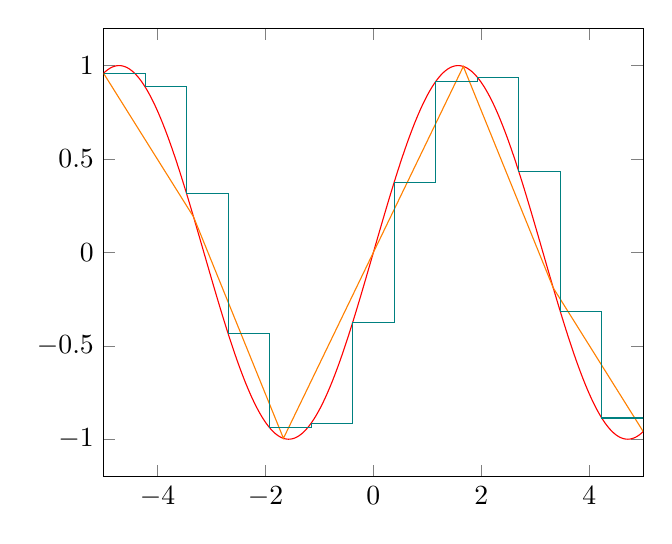
\begin{tikzpicture}
  \begin{axis}[enlarge x limits=false]
    \addplot[red,samples=500] {sin(deg(x))};
    \addplot[orange,samples=7] {sin(deg(x))};
    \addplot[teal,const plot,samples=14] {sin(deg(x))};
  \end{axis}
\end{tikzpicture}

  \caption{Beispieldiagramm 2.}
  \label{fig:eval:diag2}
\end{figure}

\begin{figure}
\centering
%%%%%%%%%%%%%%%%%%%%%%%%%%%%%%%%%%%%%%%%%%%%%%%%%%%%%%%%%
% Testdiagramm 3
%%%%%%%%%%%%%%%%%%%%%%%%%%%%%%%%%%%%%%%%%%%%%%%%%%%%%%%%%


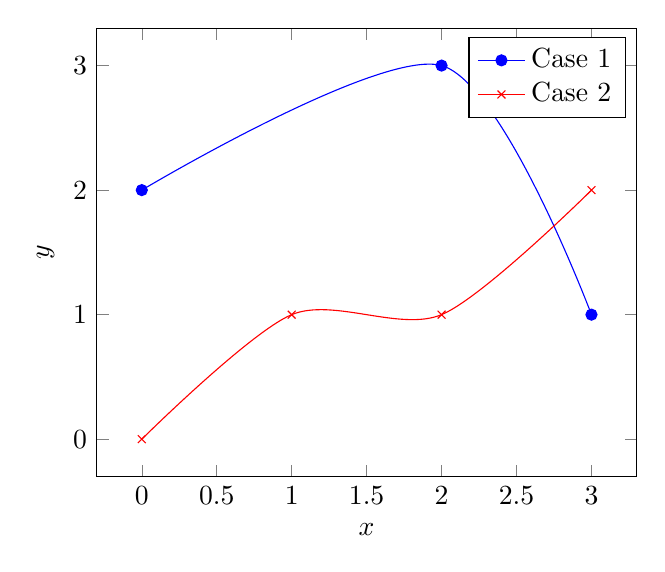
\begin{tikzpicture}
  \begin{axis}[xlabel=$x$, ylabel=$y$]
    \addplot[smooth,mark=*,blue] plot coordinates {
      (0,2)
      (2,3)
      (3,1)
    };
    \addlegendentry{Case 1}
    \addplot[smooth,color=red,mark=x]
        plot coordinates {
            (0,0)
            (1,1)
            (2,1)
            (3,2)
        };
    \addlegendentry{Case 2}
  \end{axis}
\end{tikzpicture}

  \caption{Beispieldiagramm 3.}
  \label{fig:eval:diag3}
\end{figure}

\begin{figure}
\centering
%%%%%%%%%%%%%%%%%%%%%%%%%%%%%%%%%%%%%%%%%%%%%%%%%%%%%%%%%
% Testdiagramm 4
%%%%%%%%%%%%%%%%%%%%%%%%%%%%%%%%%%%%%%%%%%%%%%%%%%%%%%%%%


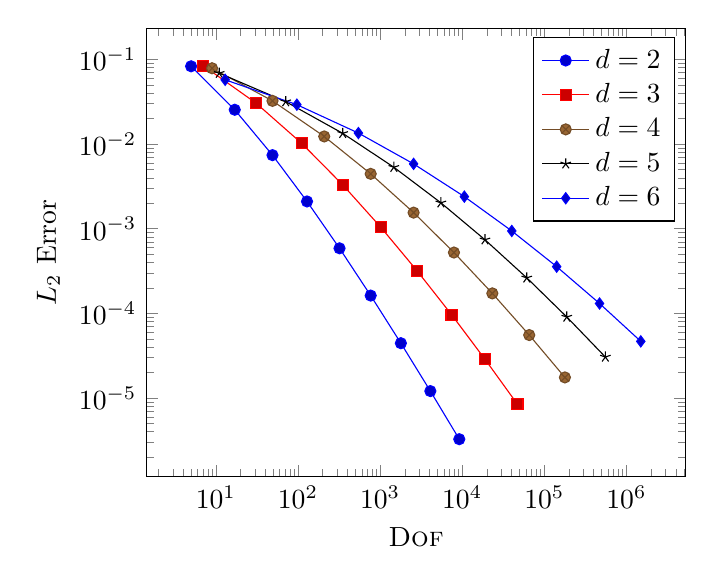
\begin{tikzpicture}
    \begin{loglogaxis}[
        xlabel=\textsc{Dof},
        ylabel=$L_2$ Error
    ]
    \axispath\draw
            (7.49165,-10.02171)
        |-  (8.31801,-11.32467)
        node[near start,left] {$\frac{dy}{dx} = -1.58$};
      \addplot plot coordinates {
        (5,     8.312e-02)
        (17,    2.547e-02)
        (49,    7.407e-03)
        (129,   2.102e-03)
        (321,   5.874e-04)
        (769,   1.623e-04)
        (1793,  4.442e-05)
        (4097,  1.207e-05)
        (9217,  3.261e-06)
    };

    \addplot plot coordinates {
        (7,     8.472e-02)
        (31,    3.044e-02)
        (111,   1.022e-02)
        (351,   3.303e-03)
        (1023,  1.039e-03)
        (2815,  3.196e-04)
        (7423,  9.658e-05)
        (18943, 2.873e-05)
        (47103, 8.437e-06)
    };

    \addplot plot coordinates {
        (9, 7.881e-02)
        (49,    3.243e-02)
        (209,   1.232e-02)
        (769,   4.454e-03)
        (2561,  1.551e-03)
        (7937,  5.236e-04)
        (23297, 1.723e-04)
        (65537, 5.545e-05)
        (178177,    1.751e-05)
    };

    \addplot plot coordinates {
        (11,    6.887e-02)
        (71,    3.177e-02)
        (351,   1.341e-02)
        (1471,  5.334e-03)
        (5503,  2.027e-03)
        (18943, 7.415e-04)
        (61183, 2.628e-04)
        (187903,    9.063e-05)
        (553983,    3.053e-05)
    };

    \addplot plot coordinates {
        (13,    5.755e-02)
        (97,    2.925e-02)
        (545,   1.351e-02)
        (2561,  5.842e-03)
        (10625, 2.397e-03)
        (40193, 9.414e-04)
        (141569,    3.564e-04)
        (471041,    1.308e-04)
        (1496065,   4.670e-05)
    };
    \legend{$d=2$\\$d=3$\\$d=4$\\$d=5$\\$d=6$\\}

    \end{loglogaxis}
\end{tikzpicture}

  \caption{Beispieldiagramm 4.}
  \label{fig:eval:diag4}
\end{figure}

\begin{figure}
  \centering
  %%%%%%%%%%%%%%%%%%%%%%%%%%%%%%%%%%%%%%%%%%%%%%%%%%%%%%%%%
% Testdiagramm 5
%%%%%%%%%%%%%%%%%%%%%%%%%%%%%%%%%%%%%%%%%%%%%%%%%%%%%%%%%


\begin{tikzpicture}
  \tikzset{ 
    every pin/.style={fill=yellow!50!white,rectangle,rounded corners=3pt,font=\tiny}, 
    small dot/.style={fill=black,circle,scale=0.3} } 
  \begin{axis}[
    x=10cm, y=0.5cm, 
    clip=false,
    ytick=\empty,
    %major x tick num=5,
    %hide y axis,
    enlargelimits=false,
    axis on top] 
    \addplot graphics [xmin=0,xmax=1,ymin=0,ymax=1, 
      % trim=left bottom right top 
      includegraphics={trim=0 9 0 8,clip}
      ] 
      {images/1d_texture.pdf}; 

\node[small dot,pin=-120:{$\frac{1}{2n}$}] at (axis description cs:0.017625,0) {}; 
\node[small dot,pin=-45:{$\frac{1}{n}$}] at (axis description cs: 0.03325,0) {}; 

  \end{axis} 
\end{tikzpicture}
  \caption{Beispieldiagramm 5. }
  \label{fig:eval:diag5}
\end{figure}
